\begin{exercise}
What is the Bellman equation for action values, that is, for $q_\pi$?
It must give the action value $q_\pi(s, a)$ in terms of the action values, $q_\pi(s_0, a_0)$, of possible successors to the state-action pair $(s, a)$.
Hint:
the backup diagram to the right corresponds to this equation.
Show the sequence of equations analogous to \eqref{eq:2.15}, but for action values.

\begin{figure}[H]
    \centering
    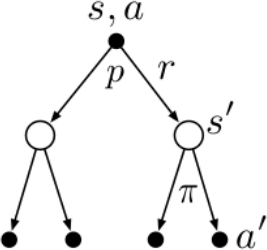
\includegraphics[width = 0.2 \textwidth]{2.17.png}
    \caption{$q_\pi$ backup diagram}
    \label{fig:2.17}
\end{figure}

\end{exercise}

\begin{solution}
  We use the law of total expectation and get:

  \begin{align*}
    q_\pi(s,a)
    &=
    \E_\pi\big[G_t \mid S_t = s, A_t = a\big]
    =
    \E_\pi\big[R_{t+1} + \gamma G_{t+1}\mid S_t = s, A_t = a\big] \\
    &=
    \sum_{s^\prime, r} p(s^\prime, r \mid s,a) \E_\pi\big[R_{t+1} + \gamma G_{t+1} \mid S_t = s, A_t = a, S_{t+1} = s^\prime, R_{t+1} = r\big]  \\
    &=
    \sum_{s^\prime, r} p(s^\prime, r \mid s,a) \Big[r + \gamma \E_\pi\big[G_{t+1} \mid S_t = s, A_t = a, S_{t+1} = s^\prime, R_{t+1} = r\big]\Big] \\
    &=
    \sum_{s^\prime, r} p(s^\prime, r \mid s,a) \Big[r + \gamma \sum_{a^\prime}\pi(a^\prime\mid s^\prime)\E_\pi\big[G_{t+1}\mid S_{t+1} = s^\prime, A_{t+1} = a^\prime \big]\Big] \\
    &=
    \sum_{s^\prime, r} p(s^\prime, r \mid s,a) \Big[r + \gamma \sum_{a^\prime}\pi(a^\prime\mid s^\prime)q_\pi(s^\prime,a^\prime)\Big]
  \end{align*}
\end{solution}
